\documentclass[12pt, letterpaper,spanish]{article}
\usepackage[letterpaper]{geometry}
\usepackage[T1]{fontenc} %para escribir con caracteres utf8 como tildes
\usepackage[utf8]{inputenc} %para escribir con caracteres utf8 como tildes
\usepackage[spanish]{babel} %para escribir con caracteres utf8 como tildes
\usepackage{lmodern} % latin modern font
\usepackage{color}
\usepackage[svgnames]{xcolor} % para hacer enfasis con colores
\usepackage{amssymb}
\usepackage{amsmath}
\usepackage{hyperref}
\usepackage{multirow}
\usepackage{array}
\usepackage{mathtools} % para el modulo
\DeclarePairedDelimiter\abs{\lvert}{\rvert}%
\DeclarePairedDelimiter\norm{\lVert}{\rVert}%
\hypersetup{
	colorlinks=true,
	linkcolor=black,
	filecolor=magenta,      
	urlcolor=cyan,
}

\usepackage{listings}
\lstloadlanguages{Python}
\definecolor{background}{rgb}{0.52, 0.52, 0.51}
\definecolor{keywords}{rgb}{1.0, 0.0, 0.5}
\definecolor{comments}{rgb}{0.75, 0.75, 0.75}
\definecolor{strings}{rgb}{0.91, 0.84, 0.42}
\definecolor{names}{rgb}{0.4, 1.0, 0.0}
\definecolor{white}{rgb}{1.0, 1.0, 1.0}
\definecolor{types}{rgb}{0.13, 0.67, 0.8}
\definecolor{numbers}{rgb}{0.54, 0.17, 0.89}

\lstdefinelanguage{PySharp}{
	keywords={method, include, if, else, elif, while, continue, break, return},
	keywordstyle=\color{keywords}\bfseries,
	ndkeywords={int, void, rider, true, false},
	ndkeywordstyle=\color{types}\bfseries,
	identifierstyle=\color{white},
	sensitive=false,
	emph={print, test, example, Rossi, curves},
	emphstyle=\color{names},
	comment=[l]{//},
	morecomment=[s]{/*}{*/},
	commentstyle=\color{comments}\ttfamily,
	stringstyle=\color{strings}\ttfamily,
	morestring=[b]',
	morestring=[b]"
}

\lstset{
	language=PySharp,
	backgroundcolor=\color{background},
	extendedchars=true,
	basicstyle=\footnotesize\ttfamily,
	showstringspaces=false,
	showspaces=false,
	numbers=left,
	numberstyle=\footnotesize,
	numbersep=9pt,
	tabsize=2,
	breaklines=true,
	showtabs=false,
	captionpos=b
}


\usepackage{amsthm} % para teoremas y lemas
\usepackage{graphicx} % para imagenes
\usepackage{titling} % para el pretitle
\usepackage{clrscode3e} % para pseudocodigos
\usepackage[stable]{footmisc} % para permitir footnotes in los encabezados

%\usepackage[cache=false]{minted} %para representar los codigos necesita config extra
%\renewcommand\theFancyVerbLine{\normalsize\arabic{FancyVerbLine}} % incrementar el tamaño de linenumbers de minted


\newtheorem{theorem}{Teorema}[subsection]
\newtheorem{corollary}{Corolario}[theorem]
\newtheorem{lemma}{Lema}[subsection]
\newtheorem{lemmacorollary}{Corolario}[lemma]
\theoremstyle{definition}
\newtheorem*{definition}{Definición}
\theoremstyle{remark}
\newtheorem*{remark}{Observación}
\renewcommand{\qedsymbol}{$\blacksquare$} % se remplaza el simbolo vacio de final de demostración
\graphicspath{ {./_static/} }

%--------------------------
% NO MODIFICAR ESTE DOCUMENTO
%--------------------------
	
\begin{document}
	
\begin{titlepage}
	\begin{center}
		
\includegraphics[width = 3cm]{escudoUH} 
	\end{center}
	\begin{center}
		Universidad de La Habana \\\vspace{0.2cm} Facultad de Matemática y Computación
	\end{center}
	\centering
	\vspace{1cm} \par
	{\scshape\Large Proyecto de \par Compilación + Inteligencia Artificial + Simulación\par}
	\vspace{5mm} \par
	{\scshape\Huge Simulador de \par un Jefe Técnico de MotoGP\par}
	\vspace{5mm} \par
	\vfill
	{\Large \textbf{Autores:} \par}
	{\large Arnel Sánchez Rodríguez \space Grupo: C312 \par}
	\href{mailto:arnelsanchezrodriguez@gmail.com}{arnelsanchezrodriguez@gmail.com}\par
	\vspace{3mm} \par
	{\large Samuel Efraín Pupo Wong \space Grupo: C312 \par}
	\href{mailto:s.pupo@estudiantes.matcom.uh.cu}{s.pupo@estudiantes.matcom.uh.cu}
	\vspace{3mm} \par
	{\large Darián Ramón Mederos \space Grupo: C312 \par}
	\href{mailto:darianrm24@gmail.com}{darianrm24@gmail.com}
	\vspace{3mm} \par
	\vfill
	{\Large 2021-2022 \par}
\end{titlepage}	
\pagebreak
\tableofcontents
\pagebreak

\section{Introducción}

	\subsection{Motociclismo de Velocidad}
	El motociclismo de velocidad es una modalidad deportiva del motociclismo disputada en circuitos de carreras pavimentados. Las motocicletas que se usan pueden ser prototipos, es decir, desarrolladas específicamente para competición, o derivadas de modelos de serie (en general motocicletas deportivas), con modificaciones para aumentar las prestaciones. En el primer grupo entran las que participan en el Campeonato Mundial de Motociclismo, y en el segundo las \emph{Superbikes}, las \emph{Supersport} y las \emph{Superstock}.
	
	Estas deben presentar una serie de características como: estabilidad, alta velocidad (tanto en recta como en paso por curva), gran aceleración, gran frenada, fácil maniobrabilidad y bajo peso.
	
	\begin{center}
		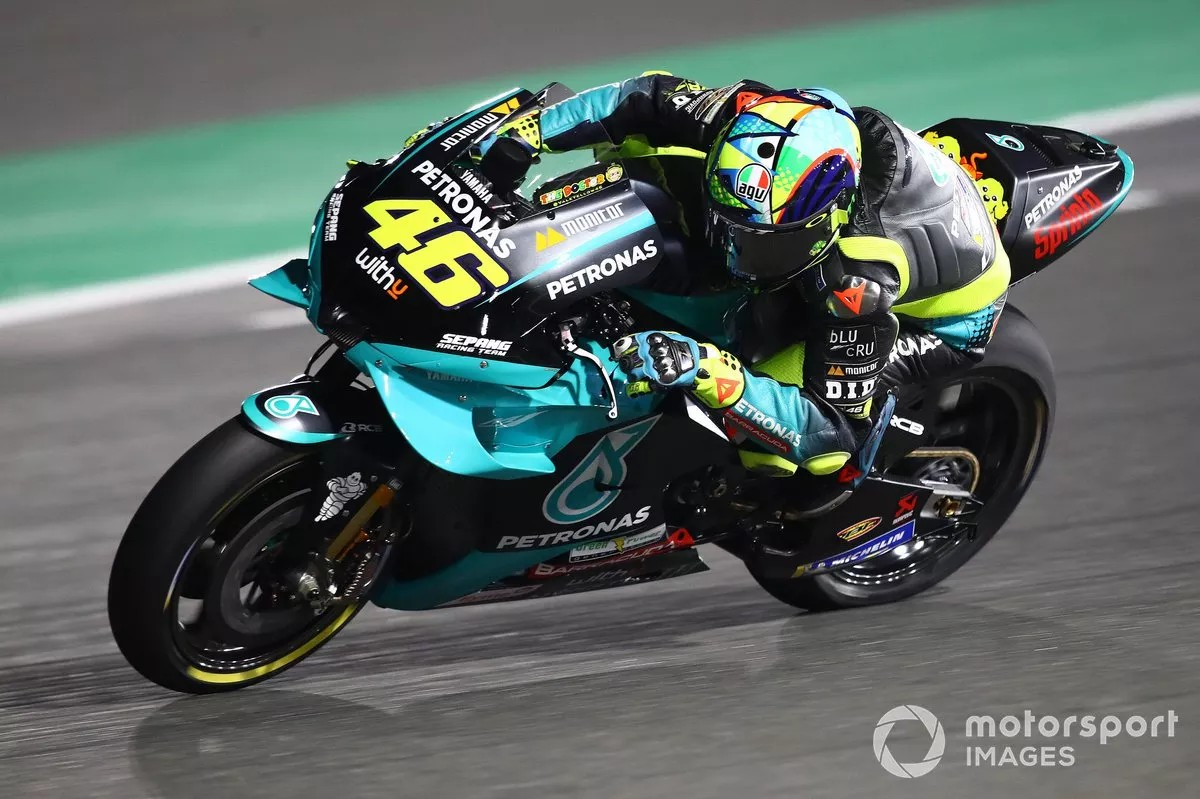
\includegraphics[width = 12cm]{imagen1} 
	\end{center}	
	
	\subsection{Estructura del Paddock}
	 En MotoGP, el \textbf{Jefe Técnico} de cada estructura se configura como una personalidad de bastante importancia dentro de un box, pues es quien se encarga de dirigir y controlar que todo funcione como un excelente engranaje que gane carreras. De igual importancia son los \textbf{Ingenieros Telemétricos}, pues son las personas que se encargan de analizar, leer y comprender todos los datos proporcionados por el piloto, así como transmitírselos al protagonista. Se trata de una figura de la que depende mucha de la información acerca de cualquier cambio realizado en la moto o asumir los puntos más fuertes de sus pilotos. Los \textbf{Mecánicos} también desempeñan un papel fundamental a la hora de construir la máquina perfecta.

	\subsection{Pista}
	Se utilizará como referencia el circuito de Misano {\footnotesize \cite{misano}}, Misano World Circuit Marco Simoncelli, autódromo localizado en la fracción de Santa Mónica, comuna de Misano Adriático (provincia de Rímini), región de Emilia-Romaña, Italia. 
	
	\begin{center}
		\includegraphics[width = 12cm]{circuito} 
	\end{center}

	\subsection{Definición del Problema}
	Se tienen varios pilotos con sus respectivas motos, las cuáles difieren entre sí en cuanto a sus prestaciones. Cada uno posee su propio método de manejo, siendo algunos más cuidadosos y otros más agresivos. La pista se encuentra influenciada por el accionar del clima, puesto que no es lo mismo el manejo durante un día soleado que bajo la lluvia. Por tanto, el resultado de un piloto se verá condicionado por la combinación de su moto, su modo de conducción, la pista y el clima.

	Sin embargo, durante la carrera las condiciones pueden variar y es necesario realizar los ajustes necesarios para que el piloto mejore su rendimiento, los cuales se harán al pasar de una sección a otra de la pista o al finalizar cada vuelta. Esto podrá hacerse utilizando un lenguaje imperativo, mediante el uso de palabras claves, para que el piloto no necesite analizar situaciones complejas y pueda concentrarse en pilotar de la forma más eficiente posible.

	De esta manera, la simulación de la carrera será dinámica, puesto que entre las vueltas podrán existir variaciones provocadas por los ajustes propuestos por el Jefe Técnico, el cuál podrá ser una persona o una IA.\par

\newpage
\section{Diseño del Sistema}
		
	\subsection{Simulación {\footnotesize \cite{conferenciasS}\cite{garcia}}}
	Se desea simular una carrera de MotoGP. Con tal fin, se utiliza una estructura agente conformada por un piloto y una moto, y una estructura ambiente formada por el clima y la pista. Se trata de un sistema multiagentes en el que dos de estos pueden interactuar entre sí, ya sea en modo ofensivo o en modo defensivo. Las variables de las distintas entidades se manipulan utilizando una escala del $1$ al $10$, donde sus valores se clasifican como: bajos (menores que $4$), medios (entre $4$ y $6$), y altos (mayores que $6$); excepto en los casos en los que se utilizan estructuras \emph{Enums} para definir los datos.
	
		\subsubsection{Ambiente}
		\textbf{El ambiente} se compone por la combinación del clima y la pista.\\

		\textbf{El clima} es simulado utilizando variables aleatorias con distribución normal, que responden a:
		\begin{itemize}
    		\item El estado del clima
    		\item La humedad
    		\item La temperatura
		\item La visibilidad
		\item La dirección e intensidad del viento
		\end{itemize}

		El uso de la distribución normal se debe a que son menos comunes los climas extremos. Nótese que la escala utilizada permite esta configuración.

		Una función probabilística es la encargada de lanzar un evento de cambio de clima, generando nuevo estado de este. Además, sus parámetros se varían cada vez que termina una vuelta de la carrera. Es importante señalar que estas variables se encuentran enlazadas bajo ciertas circustancias, como es el caso de un aumento de la humedad cuando comienza a llover. \\ \\

		\textbf{La pista} posee:
		\begin{itemize}
    		\item El nombre
		\item La longitud total
		\item La lista de las secciones que la componen
		\end{itemize}

		Donde cada \textbf{sección} está formada por:
		\begin{itemize}
    		\item El nombre
    		\item La longitud
		\item La velocidad máxima alcanzable (sin accidentarse)
		\item La orientación cardinal
		\item El tipo de sección (curva o recta)
		\item Si tiene un equivalente en boxes y, en caso de tenerlo, su longitud.
		\end{itemize}
		
		El circuito de Misano es el escogido por defecto para la competición. Sin embargo, es posible reestructurar la pista para crear una experiencia diferente o, incluso, generar una nueva pista de manera aleatoria automáticamente. Mas debemos asegurarnos de que estas nuevas creaciones sean estructuras válidas.

		El método de reestructuración intercambia las curvas o rectas con otras secciones de su mismo tipo y su misma orientación cardinal. De este modo, se asegura de que solo se varíe el orden de estas y no se pierdan las propiedades que hacen al circuito cerrado.

		Por otro lado, generar una nueva pista de manera aleatoria automáticamente es una problemática topográfica de un mayor nivel de complejidad. Como solución factible simplificada, se genera una línea poligonal de secciones, que parte de un punto y se expande variando su orientación. 

		La longitud de cada sección es generada utilizando una variable aleatoria, donde los mayores valores tienen una menor probabilidad. Luego, atentiendo a dicha longitud, la velocidad máxima alcanzable se calcula por rangos, agregando incertidumbre mediante probabilística con distribución uniforme.

		Cuando la longitud total excede el mínimo necesario, se redirige la orientación de las nuevas secciones en sentido cardinal opuesto al inicial. Esta línea es abierta, pero su punto final está orientado en sentido inverso al punto inicial. Luego, tomando una copia exacta de esta y rotándola $180^0$, se puede crear una figura poligonal cerrada con simetría central, la cual responde a las condiciones necesarias de una pista.

		\subsubsection{Agentes}
		Un agente está compuesto por un piloto y su moto. \\

		\textbf{El piloto} está conformado por:
		\begin{itemize}
    		\item El nombre
    		\item La habilidad de pasar por la curva y por la recta
    		\item La probabilidad de caerse de la moto
    		\item La independencia (probabilidad de ignorar órdenes)
    		\item La agresividad
    		\item La pericia
		\end{itemize}

		Los valores de estas características oscilan entre $1$ y $10$, pero son divididos por potencias de $10$, con el objetivo de que respondan a probabilidades generadas por variables aleatorias con distribución uniforme. 
		
		Las habilidades de manejo son tomadas en cuenta para el paso por las distintas secciones de la pista. La independencia da la probabilidad de que el piloto tome sus propias decisiones, ignorando las orientaciones dadas por el \textbf{Jefe Técnico}. Mientras, la agresividad es la tendencia a ejercer acciones más riesgosas y la pericia, la capacidad para salir airoso de ellas. \\ \\

		\textbf{La moto} posee:
		\begin{itemize}
    		\item La marca
    		\item El modelo
    		\item La velocidad máxima alcanzable
    		\item El peso
    		\item El tipo de neumáticos (lisos o de lluvia)
    		\item Los frenos
    		\item La rigidez del chasis
    		\item La probabilidad de romperse
    		\item La probabilidad de que exploten los neumáticos por desgaste
		\end{itemize}

		Las propiedades de las motos influyen en el manejo de sus pilotos y, por tanto, en el resultado de estos en la carrera. Sobreexplotarlas lleva consigo un mayor desgaste, lo que provoca un aumento en la probabilidad de una caída. \\ \\ 

		Además del piloto y su moto, un \textbf{agente} está compuesto por variables que responden a su desempeño en la carrera:
		\begin{itemize}
    		\item La velocidad y la aceleración actuales
    		\item El tiempo de la vuelta y el tiempo total
    		\item La sección de la pista en la que se encuentra
    		\item La posición en el ranking
    		\item La entrada a boxes (el piloto cambia de moto)
    		\item Si sufrió o provocó un accidente (se cayó o derribó a otro piloto)
		\end{itemize}

		\subsubsection{La carrera}
		El \emph{ranking} de la carrera permite conocer las posiciones de los pilotos mientras corren en sus motos, para así premiar al ganador.

		Inicialmente, los agentes parten en un orden por defecto calculado de manera aleatoria, asumiendo que este se alcanzó el día anterior en las clasificaciones. El comienzo de la carrera se hace desde la primera sección de la pista, y tomando un piloto a la vez se calculan sus interacciones, haciendo que este avance.

		 Las acciones que el agente puede ejecutar en un instante determinado dependen de las variables del ambiente, las del propio agente, y las de sus rivales inmediatos hacia adelante y hacia atrás. Analizando las consecuencias de la acción escogida (acelerar, frenar, doblar, ir a boxes o luchar por la posición), se considera si fue correcta y sobrepasó la sección o, en caso contrario, sufrió un accidente. 

		De efectuar ataque (intentar superar a otro piloto) o defensa (evitar ser superado), se provoca una interacción con otros agentes. Si un ataque es satisfactorio, se intercambian las posiciones en el  \emph{ranking}, sino su tiempo en la carrera sufre una penalización. Existen variables probabilísticas que calculan si el piloto comete un error y debe abandonar la carrera, provoca la salida de otro piloto, o ambos. Tomando su aceleración, se puede calcular su nueva velocidad y el tiempo que demora en llegar a una nueva sección.

		Sin embargo, es necesario decidir la forma más acertada de otorgarle el turno al próximo piloto. Para ello se utiliza una cola con prioridad, donde los agentes están ordenados por sus tiempos en la carrera. Esto se debe a que, al pasar su turno, el tiempo que poseen es el que demorarán en llegar a la nueva sección. Por tanto, esto permite darle el turno al más rápido primero, pues se supone que debe avanzar más veloz que los que demoran más.

		Dicho sistema (cola con prioridad por tiempo) permite tener varios agentes en diferentes secciones, corriendo a distintas velocidades. Cada vez que un piloto tiene su turno y logra continuar, se actualizan las variables que lo componen. En caso de que no esté solo en su sección y su tiempo teórico sea menor que quien le antecede, se reajustan las posiciones utilizando ataque/defensa. Al pasar por la meta, se muestra el \emph{ranking} según van completando las vueltas, hasta que se completa la carrera.

		Los parámetros de las distintas entidades pueden interactuar entre ellos, lo que trae determinadas consecuencias, algunas positivas y otras negativas. Dado que dichas interacciones se producen en mayor o menor medida, después de varias pruebas se obtuvo una escala que se puede considerar funcional, puesto que se acerca a los resultados de una carrera verdadera. 

		Para lograr un mayor realismo, se hace una primera variación de parámetros para adaptar a las entidades a las condiciones climatológicas del momento; luego, en cada cambio de vuelta se modifica el clima y se reajustan los parámetros de acuerdo las nuevas condiciones climatológicas.

		Los agentes reciben cada variación del ambiente y analizan qué modificaciones realizar para adaptarse. Asimismo, las interacciones entre dos de estos provocan cambios en sus condiciones. Nótese que en un momento dado, una interacción puede generar una reacción en cadena que provoque una serie de cambios en varios agentes que compiten directamente entre sí. Una variable probabilística, influida por las habilidades de los pilotos en cuestión, sirve para obtener el resultado de un ataque o una defensa.

	\newpage

	\subsection{Inteligencia Artificial  {\footnotesize \cite{conferenciasIA}\cite{russell}}}
	Una inteligencia artifical es la encargada de elegir las acciones a realizar por cada agente, con el fin de tomar las mejores decisiones para alcanzar el máximo rendimiento. Para su implementación se utilizan: \textbf{Sistemas Expertos} generados mediante el uso de un procedimiento declarativo/imperativo, utilizando la biblioteca \textbf{PyKE}{\footnotesize \cite{pyke}} de \textbf{Python}; y \textbf{heurísticas}. También se emplean variables probabilísticas para crear incertidumbre, es decir, la respuesta de la IA ante la misma situación puede variar: es \textbf{no determinista}.
	
	Se emplea como base de conocimiento el conjunto de variables, antes expuestas, que forman parte de la simulación y que influyen en el desempeño:
	\begin{itemize}
		\item Las condiciones del clima
		\item Las características de la sección
		\item Las habillidades del piloto
		\item Las propiedades de la moto
		\item El estado del agente
	\end{itemize}
	
		\subsubsection{Configuración de la moto}
		El primer sistema se encarga de escoger la mejor configuración de la moto. De este modo, atendiendo a las condiciones iniciales de la carrera (que serán los hechos), la IA podrá tomar decisiones atendiendo a las reglas definidas. Al ser declarativas, las determinaciones tomadas se obtendrán mediante \emph{match} hechos-reglas. \\
		
		\textbf{Los hechos} se presentan mediante lógica difusa y n-valente:
		\begin{lstlisting}[language={Python}, label={Script}]
		weather(Sunny)
		humidity(2)
		wind_intensity(7)
		wind_direction(3)
		\end{lstlisting}
	
		\textbf{Las reglas} se formulan del modo:
		\begin{lstlisting}[language={Python}, label={Script}]
		slick
		    use select_type(Slick)
		    when
		        moto_facts.weather($ans_1)
		        check $ans_1 != "Rainy"
		        moto_facts.humidity($ans_2)
		        check $ans_2 <= 6
		
		soft
		    use select_tires(Soft)
		    when
		        moto_facts.wind_intensity($ans_1)
		        check $ans_1 > 6
		        moto_facts.wind_direction(3)
		\end{lstlisting}

		Tomando este ejemplo, el sistema analiza los hechos y las reglas permitiendo llegar a la decisión de tomar neumáticos \emph{Slick\_Soft} (lisos suaves). Luego, consultando los resultados obtenidos por PyKE, mediante Python de manera imperativa será posible la interacción con la simulación de la carrera. En este caso, se utiliza para generar la selección un \emph{Enum}:
		\begin{lstlisting}[language={Python}, label={Script}]
		class Tires(Enum):
		    Slick_Soft = 0
		    Slick_Medium = 1
		    Slick_Hard = 2
		    Rain_Soft = 3
		    Rain_Medium = 4
		\end{lstlisting}

		El resto de los parámetros de la moto no son modificados, puesto que se asume que la configuración por defecto es la óptima. No así con los neumáticos, de los cuáles depende mucho el rendimiento, atendiendo a las variaciones del clima.
	
		\subsubsection{Selección de acciones}
		Un segundo sistema se emplea para escoger la acción que debe ejecutar el piloto, atendiendo a las condiciones de la carrera:
		\begin{itemize}
			\item Aumentar/disminuir/mantener la velocidad
			\item Doblar
			\item Ir a \emph{pits}
			\item Atacar/defender
			\item Combinaciones de todas las anteriores
		\end{itemize}		

		(Ejemplo: Aumentar la velocidad + Doblar + Atacar) \\
	
		En este caso, se utiliza el mismo método antes expuesto, declarativo/imperativo con el uso de PyKE.

		Hechos:
		\begin{lstlisting}[language={Python}, label={Script}]
		speed(Lower)
		section(Straight)
		slick_tires(True)
		weather(Cloudy)
		humidity(6)
		nearest_forward(60)
		nearest_behind(-60)
		\end{lstlisting}

		Reglas:
		\begin{lstlisting}[language={Python}, label={Script}]
		speed_up
 		    use select_action(SpeedUp)
  		    when
		        action_facts.speed("Lower")

		keep_speed
		    use select_action(KeepSpeed)
		    when
		        action_facts.speed("Same")

		brake
		    use select_action(Brake)
		    when
		        action_facts.speed("Higher")

		turn
		    use select_action(Turn)
		    when
		        action_facts.section("Curve")
		\end{lstlisting}
	
		Las acciones obtenidas son combinadas con el fin de generar una respuesta compuesta mediante un \emph{Enum}:	
		\begin{lstlisting}[language={Python}, label={Script}]
		class AgentActions(Enum):
		    SpeedUp = 0
		    KeepSpeed = 1
		    Brake = 2
		
		    SpeedUp_Turn = 3
		    KeepSpeed_Turn = 4
		    Brake_Turn = 5
		
		    SpeedUp_Pits = 6
		    KeepSpeed_Pits = 7
		    Brake_Pits = 8
		
		    SpeedUp_Turn_Pits = 9
		    KeepSpeed_Turn_Pits = 10
		    Brake_Turn_Pits = 11
		
		    SpeedUp_Attack = 12
		    KeepSpeed_Attack = 13
		    Brake_Attack = 14
		
		    ...
		
		    SpeedUp_Turn_Pits_Defend = 33
		    KeepSpeed_Turn_Pits_Defend = 34
		    Brake_Turn_Pits_Defend = 35
		\end{lstlisting}

		Las condiciones del ambiente y del agente en cuestión determinan sus acciones:
		\begin{itemize}
			\item Debe doblar en caso de que la sección sea curva
			\item Debe acelerar si su velocidad no supera a la máxima permitida (sin sufrir un accidente), o viceversa
			\item Debe ir a boxes en caso de que el clima le obligue a cambiar los neumáticos
			\item Puede atacar o defender en caso de que su rival más cercano esté lo suficientemente cerca (menos de $1$ segundo de distancia), o en caso de reacción
		\end{itemize}

		Sin embargo, en función inversa a la pericia del piloto, existe una probabilidad de que este se equivoque y deba abandonar la carrera.
		
	
		\subsubsection{Selección de la aceleración}
		Una heurística, apoyada en fórmulas de Física y probabilidades, es la encargada de escoger la mejor aceleración en una sección dada de la pista, con el objetivo de alcanzar la mayor velocidad posible sin accidentarse. 

		Primeramente, se calcula la aceleración máxima alcanzable:
		\begin{equation}\label{eq:a_max}
		a_{max}=\frac{v_{max}^{2} - v^{2}}{2 \cdot x}
		\end{equation}

		Donde $v$ es la velocidad actual del piloto, $v_{max}$ es el mínimo entre la velocidad máxima alcanzable por la moto y en la sección, y $x$ es la longitud de dicha sección.

		Mas no siempre es posible alcanzar esta aceleración teórica, pues influyen las condiciones del clima y de la moto, así como también las habilidades del piloto. Entonces, se establece un sistema de penalizaciones que disminuyen el valor obtenido, en caso de que las circunstancias no sean óptimas:
		\begin{itemize}
			\item El clima no es el mejor (humedad y temperatura muy altas o muy bajas, baja visibilidad, viento intenso)
			\item Los frenos y la rigidez del chasis no son apropiados
			\item La habilidades del piloto en las rectas y las curvas no son buenas
		\end{itemize}

		Sin embargo, un piloto más agresivo puede tomar mayores riesgos e ignorar ciertas penalizaciones con el fin de acercarse a la aceleración máxima. Esta probabilidad se ve influida por las características del piloto, aumentando también en el caso de encontrarse en una pugna de posición (ataque o defensa). Por tanto, el valor hallado es no determinista.

		Luego, se calcula la nueva velocidad del agente:
		\begin{equation}\label{eq:v}
		v=\sqrt{v_{0}^{2} + 2 \cdot a \cdot x}
		\end{equation}

		Y con esta, el tiempo demorado en superar la sección:
		\begin{equation}\label{eq:t_1}
		t=\frac{v - v_{0}}{a}
		\end{equation}

		En caso de que la aceleración fuera $0$, la velocidad no varía y se utiliza solamente:
		\begin{equation}\label{eq:t_2}
		t=\frac{x}{v}
		\end{equation}

		La diferenciación entre ambas fórmulas es importante, pues no es lo mismo el Movimiento Rectilíneo Uniforme (MRU) [\ref{eq:t_2}] que el Movimiento Rectilíneo Uniformemente Acelerado (MRUA), o Desacelerado [\ref{eq:v}, \ref{eq:t_1}].

		De esta manera, se actualizan los parámetros del agente; siendo los más importantes el tiempo de la vuelta y de la carrera, que se nutren del tiempo recién calculado. Los resultados obtenidos son incorporados a la simulación para continuar con esta, de ellos depende si el piloto triunfa o sufre un accidente que lo saque de la competencia.

\newpage

\section{Definición del Lenguaje {\footnotesize \cite{conferenciasC}\cite{ullman}}}
	\subsection{Introducción a PySharp (P\#)}

		\subsubsection{Estructura del Programa}
		Los archivos de \textbf{P\#} suelen tener la extensión de \textbf{.pys}. Sus conceptos organizativos clave son programas, tipos y miembros. Los programas constan de un archivo fuente y declaran tipos y miembros. Las motocicletas y los motociclistas son ejemplos de tipos. Los métodos y propiedades son ejemplos de miembros.
	
	\subsubsection{Tipos y Variables}
	En P\# solo existen tipos de valor, no hay de referencia. Por tanto, todas las variables contienen directamente sus datos, cada una tiene su propia copia y no es posible que las operaciones en una afecten a otra.

	\begin{center}
		\begin{tabular}{| c | c | m{5cm} | }
			\hline
			Categoría & Tipo & Descripción \\ \hline
			\multirow{5}{*}{Tipos} & \multirow{4}{*}{Tipos Simples} & Entero con signo: int \\ \cline{3-3}
			&  & Punto flotante IEEE: double \\ \cline{3-3}
			&  & Booleanos: bool \\ \cline{3-3}
			&  & Cadenas Unicode: string \\ \cline{2-3}
			& Tipos que aceptan valores NULL & Extensiones de todos los demás tipos de valor con un valor nulo \\ \hline
		\end{tabular}
	\end{center}

	\subsubsection{Expresiones}
	Las expresiones se construyen a partir de operandos y operadores. Los operadores de una expresión indican qué operaciones aplicar a los operandos. Los ejemplos de operadores incluyen: +, -, * y /. Ejemplos de operandos son: literales, variables y expresiones.

	\begin{center}
		\begin{tabular}{| c | c | m{5cm} | }
			\hline
			Categoría & Expresión & Descripción \\ \hline
			\multirow{2}{*}{Primaria} & x(...) & Invocación de método \\ \cline{2-3}		
			\multirow{4}{*}{Multiplicativa} & x $\ast$ y & Multiplicación \\ \cline{2-3}
			& x / y & División \\ \cline{2-3}
			& x \% y & Resto \\ \cline{2-3} 
			& x $\ast\ast$ y & Exponenciación \\ \hline
			\multirow{2}{*}{Aditiva} & x + y & Adición y concatenación de strings \\ \cline{2-3}
			& x - y & Substracción \\ \hline
			\multirow{4}{*}{Relacionales} & x <\;y & Menor que \\ \cline{2-3} 
			& x >\;y & Mayor que \\ \cline{2-3}
			& x <= y & Menor o igual que \\ \cline{2-3} 
			& x >= y & Mayor o igual que \\ \hline
			\multirow{2}{*}{Igualdad} & x == y & Igual \\ \cline{2-3} 
			& x != y & Distinto \\ \hline 
			Condicionales AND & x \&\& y & Evalúa y si y sólo si x es verdadera \\ \hline
			Condicionales OR & x || y & Evalúa y si y sólo si x es falsa \\ \hline
			Condicionales XOR & x $\wedge$ y & \\ \hline
			\multirow{2}{*}{Asignación} & x = y & Asignación \\ \cline{2-3}
			& x op= y & Asignación compuesta; los operadores admitidos son *= /= \%= **= += -= \&\&= ||= \textasciicircum{}= \\ \hline
		\end{tabular}
	\end{center}

	\subsubsection{Declaraciones}
	Las acciones de un programa se expresan mediante declaraciones. P\# admite varios tipos diferentes de declaraciones, algunas de las cuales se definen en términos de declaraciones integradas.
	
	Un \textbf{bloque} permite escribir múltiples declaraciones en contextos donde se permite una sola declaración. Un bloque consta de una lista de declaraciones escritas entre los delimitadores \textbf{\{} y \textbf{\}}.
	
	Las sentencias de \textbf{declaración} se utilizan para declarar variables, valga la redundancia.
	
	\begin{lstlisting}[language={PySharp}]
		method void example() {
			int a = 1;
		}
	\end{lstlisting}
	
	Las \textbf{declaraciones de expresión} se utilizan para evaluar expresiones. Aquellas que se pueden usar como declaraciones incluyen invocaciones de métodos, asignaciones que usan \textbf{=} y los operadores de asignación compuesta.
	
	\begin{lstlisting}[language={PySharp}]
		method int example() {
			int a = 1;
			return a + 2;
		}
	\end{lstlisting}
	
	La \textbf{instrucción de selección} se utiliza para elegir una de varias declaraciones posibles para su ejecución, en función del valor de alguna expresión. Este es el caso de la sentencia \textbf{if}-\textbf{else}.
	
	\begin{lstlisting}[language={PySharp}]
		method int example(int a) {
			if (a < 5) {
				return a;
			}
			else {
				return a % 5;
			}
		}
	\end{lstlisting}
	
	La \textbf{instrucción de iteración} se utiliza para ejecutar repetidamente una instrucción incorporada. Este es el caso de \textbf{while}.
	
	\begin{lstlisting}[language={PySharp}]
		method int example(int a) {
			while (a > 5) {				
				a -= 1;
			}
			return a;
		}
	\end{lstlisting}
	
	Las \textbf{sentencias de salto} se utilizan para transferir el control. En este grupo están las declaraciones de \textbf{break}, \textbf{continue} y \textbf{return}.
	
	\begin{lstlisting}[language={PySharp}]
		method int example() {
			x = 10
			while (true) {				
				if (x < 100) {
					x += 10;
					continue;
				}
				else {
					break;
				}
			}
			return 0;
		}
	\end{lstlisting}
	
	\subsubsection{Tipos especiales}
	Los \textbf{tipos especiales} son los elementos más importantes de P\# y constituyen estructuras de bloques compuestas por acciones (métodos). Estos proporcionan definiciones para casos de, por ejemplo, motociclistas o motocicletas. Su declaración comienza con un encabezado que especifica qué tipo se va a crear y el nombre que se le dará a esta instancia. Luego aparece cuerpo, que consiste en una lista de declaraciones de miembros escritas entre los delimitadores \textbf{\{} y \textbf{\}}.
	
	\begin{lstlisting}[language={PySharp}]
		rider Rossi() {
			method int select_action() {    
				return 0;
			}
			method int select_acceleration(){
				...
			}
			...
		}
	\end{lstlisting}
	\subsubsection{Métodos}
	Un \textbf{método} es un miembro que implementa un cálculo o acción que se puede realizar por un tipo especial. Posee una lista de \textbf{parámetros}, que representan valores de variables pasadas a este, y un tipo de retorno, que especifica el tipo de valor calculado y devuelto, el cual es nulo si no devuelve ninguno.

	\subsubsection{Parámetros}
	Los \textbf{parámetros} se utilizan para pasar valores de variables a métodos. Estos obtienen sus valores reales de los \textbf{argumentos} que se especifican cuando se invoca al método en el que se encuentran. Las modificaciones de un valor de parámetro no afectan el argumento que se pasó a través d este.
	
	\subsubsection{Cuerpo del método y variables locales}
	El cuerpo de un método especifica las declaraciones que se ejecutarán cuando se invoca al método. Este puede declarar variables que son específicas de dicha invocación, las cuales se denominan variables locales. Una declaración de variable local especifica un nombre de tipo, un nombre de variable y un valor inicial.
	
	\subsubsection{Operadores}
	Un \textbf{operador} es un miembro que define el significado de aplicar un operador de expresión particular. Se pueden definir solamente operadores binarios.\par
	
	\textbf{Operadores Binarios:}
	\begin{lstlisting}[language={PySharp}]
		3+5
		true && false
	\end{lstlisting}
	
	\subsubsection{Análisis Léxico}
	\textbf{input}\par
	: input\_element* new\_line\par
	| directive\par
	; \\
	
	\textbf{input\_element}\par
	: whitespace\par
	| comment\par
	| token\par
	; \\ \\
	
	\underline{\textbf{Fin de línea}}\par
	\textbf{new\_line}\par
	: '<Caracter de retorno (U+000D)>'\par
	| '<Caracter de avance de línea (U+000A)>'\par
	; \\
	
	\textbf{whitespace}\par
	: '<Cualquier personaje con clase Unicode Zs>'\par
	| '<Caracter de tabulación horizontal (U+0009)>'\par
	; \\ \\
	
	\underline{\textbf{Comentarios}}\par
	\textbf{comment}\par
	: '\#' comment\_section '\#'\par
	; \\ \\
	
	\underline{\textbf{Tokens}}\par
	\textbf{token}\par
	: identifier\par
	| keyword\par
	| literal\par
	| operator\_or\_punctuator\par
	; \\ \\
	
	\underline{\textbf{Identificadores}}\par
	\textbf{identifier}\par
	: '<Un identificador que no es una palabra clave>'\par
	| identifier\_start\_character identifier\_part\_character*\par
	; \\
	
	\textbf{identifier\_start\_character}\par
	: letter\_character\par
	| '<Caracter guión bajo (U+005F)>'\par
	; \\
	
	\textbf{identifier\_part\_character}\par
	: letter\_character\par
	| decimal\_digit\par
	| '<Caracter guión bajo (U+005F)>'\par
	; \\
	
	\textbf{letter\_character}\par
	: uppercase\_letter\_character\par
	| lowercase\_letter\_character\par
	; \\
	
	\textbf{uppercase\_letter\_character}\par
	: 'A' | 'B' | 'C' | 'D' | 'E' | 'F' | 'G' | 'H'\par 
	| 'I' | 'K' | 'L' | 'M' | 'N' | 'O' | 'P' | 'Q'\par 
	| 'R' | 'S' | 'T' | 'V' | 'X' | 'Y' | 'Z'\par    
	; \\
	
	\textbf{lowercase\_letter\_character}\par
	: 'a' | 'b' | 'c' | 'd' | 'e' | 'f' | 'g' | 'h'\par 
	| 'i' | 'k' | 'l' | 'm' | 'n' | 'o' | 'p' | 'q'\par
	| 'r' | 's' | 't' | 'v' | 'x' | 'y' | 'z'\par
	; \\
	
	\textbf{decimal\_digit}\par
	: '0' | '1' | '2' | '3' | '4'\par 
	| '5' | '6' | '7' | '8' | '9'\par
	; \\ \\
	
	\underline{\textbf{Palabras Claves}}\par
	\textbf{keyword}\par        
	: 'bike'\par     
	| 'bool'\par
	| 'break'\par
	| 'continue'\par 
	| 'double'\par
	| 'elif'\par
	| 'else'\par
	| 'environment'\par
	| 'false'\par
	| 'if'\par
	| 'int'\par
	| 'method'\par
	| 'null'\par
	| 'return'\par
	| 'rider'\par
	| 'string'\par
	| 'true'\par
	| 'void'\par
	| 'while'\par
	; \\ \\
	
	\underline{\textbf{Literales}}\par
	\textbf{literal}\par
	: boolean\_literal\par
	| integer\_literal\par
	| double\_literal\par
	| string\_literal\par
	| null\_literal\par
	; \\ \\
	
	\underline{\textbf{Literales Booleanos}}\par
	\textbf{boolean\_literal}\par
	: 'true'\par
	| 'false'\par
	; \\ \\
	
	\underline{\textbf{Literales Enteros}}\par
	\textbf{integer\_literal}\par
	: decimal\_digit\par
	; \\ \\
	
	\underline{\textbf{Literales flotantes}}\par
	\textbf{double\_literal}\par
	: decimal\_digit+ '.' decimal\_digit+\par
	; \\ \\
	
	\underline{\textbf{Literales de Cadenas}}\par
	\textbf{string\_literal}\par
	: '\"' string\_literal\_character* '\"'\par
	; \\
	
	\textbf{string\_literal\_character}\par
	: '<Cualquier caracter, excepto " (U+0022)'\par
	; \\ \\
	
	\underline{\textbf{Literales Nulos}}\par
	\textbf{null\_literal}\par
	: 'null'\par
	; \\ \\
	
	\underline{\textbf{Operadores y signos de puntuación}}\par		
	\textbf{operator\_or\_punctuator}\par
	: '\{' \par
	| '\}' \par
	| '[' \par
	| ']' \par
	| '(' \par
	| ')' \par
	| '.' \par
	| ',' \par  
	| ':' \par
	| ';' \par
	| '+' \par
	| '-' \par
	| '*' \par
	| '/' \par
	| '\%' \par
	| '**' \par
	| '=' \par
	| '<' \par
	| '>' \par
	| '\&\&' \par
	| '||' \par
	| '==' \par
	| '!=' \par
	| '<=' \par
	| '>=' \par
	| '+=' \par
	| '-=' \par
	| '*=' \par
	| '/=' \par
	| '\%=' \par
	| '**=' \par
	| '\&\&=' \par
	| '||=' \par
	| '\textasciicircum{}=' \par
	
	\subsection{Explicación de la Implementación}
        Para crear nuestra gramática nos apoyamos en los lenguajes Python y CSharp, de ahi el nombre de nuestro DSL PSharp. Luego de tener los tokens resultantes del tokenizer, acordamos quée tendríamos como una línea e implementamos el metodo split\_lines , el cual
        recibe los tokens y los convierte en líneas, estas líneas son pasadas al parser.

        El parser que decidimos desarrolar fue el parser LL, lo primero que hicimos fueron las producciones, donde decidimos como serían correctas sintácticamente nuestras líneas.Las producciones generan todas las posibles cadenas válidas para nuestro lenguaje y no existen cadenas que son generadas por nuestra grámatica que no pertenezcan a nuestro lenguaje.De esta forma con una gramática válida empezamos al proceso de parsing. Nuestro parser necesitó un método hacer\_first primeramente para hacer los first de cada cadena posible de nuestra gramatica, luego llamamos un método auxiliar calcular\_first\_restantes el cual tiene la función de calcular los first de los no terminales que aún no lo tienen calculado .Nos hace falta guardar los first de los no terminales porque los necesitamos para hallar los follows en el método hacer\_follow. Luego de invocar a hacer\_follow debemos invocar un método auxiliar completar\_follows el cual se encarga de satisfacer la regla de los follows que dice que el follow de la cabeza de la produccion es subconjunto del follow del ultimo no terminal, si el último no terminal puede ser el último elemento de la producción.

        Teniendo los first y los follows construimos la tabla LL(1) mediante el método construir\_tabla\_LL. Al tener la tabla ya podemos comprobar que nuestra gramática no es ambigua, siempre existe solo una producción que aplicar. Luego creamos el método parsear al que hay que pasarle todas las líneas de nuestro código una por una , este realiza la comprobación sintáctica y en este mismo método vamos a ir creando nuestro AST para luego hacer el chequeo semántico. Para crear el AST utilizamos métodos como CreaNododExpresion,  CreaNodoCondicion, CreaNododFuncion, EligeTipoDdeclaracion, entre muchos otros declarados en la clase Parser. 

        Nuestro AST tiene un nodo por cada declaración que se puede realizar en el código. Tiene un nodo para una definición de función, una 
        definición de variables, redefinición de variables, If, WHile, Rider, Bike, Return. En cada uno de estos nodos si existe un ámbito como es el caso del nodo If, el While, los tipos rider, bike, environment y la definición de función cada uno de estos nodos tienen como atributo un tipo de nodo Program, el cual posee una lista de declaraciones y por lo tanto en él se pueden guardar la lista de declaraciones que se haga en el ámbito.

        Explicada la estructura del AST pasamos al chequeo semántico sobre este. Hacemos 3 recorridos sobre el AST, el primero para validar cada nodo.Un nodo es válido si todo lo que tiene guardado en sus atributos que es dependiente del contexto puede ser utilizado desde ese contexto y de la forma que se quiere. Decimos esto porque por ejemplo, las variables solo se pueden redefinir en el contexto en que fueron definidas. Decir que cada vez que creamos una función o un tipo creamos un contexto que responde a dicho nodo. Todo lo que se defina en dicho ámbito pertenece a su contexto específicamnete, no importa si se define dentro de un
        while o dentro de un If. En resumen los contextos en nuestro programa funcionan como en python con la particularidad de que no tenemos variables globales, si quieres redefinir una variable debes hacerlo en el contexto donde fue definida y solo se crea un nuevo contexto cuando se crea una función fuera de un tipo o cuando se crea un tipo. Destacar que las funciones definidas dentro de los tipos no crean un contexto específico para ellas, sino que su contexto es el mismo que el de el tipo, y no se le pueden pasar parámetros a las que pueden ser utilizadas luego en la simulación.

        Volviendo al AST, hacemos una segunda pasada, en esta pasada verificamos los tipos,en los nodos en que hay expresiones inducimos el tipo. Decir que una expresión para nosotros puede ser una expresión aritmética, un bool, o un string, podemos incluir variables y llamado a función en una expresión. La tercera pasada la hacemos para evaluar nuestros nodos. Si encontramos un nodo Def\_Fun no lo evaluamos, una definición de función se evalúa cuando se llama a la función.

        Cuando se crea un tipo se importan las variables que puede tener ese tipo en la simulación y las que podría utilizar. Estas variables están predefinidas, por lo tanto se pueden redefinir, pero una definición de otra variable con un nombre igual al de alguna de estas variables predefinidas arrojaría un error, ya que existe una variable en ese contexto con ese nombre dentro del tipo. Dentro de cada tipo se pueden definir las funciones que el jefe técnico decida pero hay algunas funciones con nombres claves como son la función select\_configuration en un tipo Bike, las funciones select\_acceleration y select\_action en un tipo rider y la función probability\_change\_weather en un tipo environment. El objetivo de select\_configuration es seleccionar el tipo de gomas dadas las características de la moto y por tanto modificar la variable tires del contexto del tipo, la cual utilizará el simulador, esta función debe ser void, select\_action debe retornar un valor entero y es la encargada de elegir que acción realizara el piloto. La función select\_acceleration debe ser void y su objetivo es actualizar la aceleración de un agente. Las variables dentro de los tipos se actualizan justo antes de que la simulación utilice las funciones claves, para eso cada tipo tiene un método refreshContext que es quien se encarga de actualizar las variabes. Las variables que se pueden utilizar dentro de un tipo Bike son los atributos de dicha moto y las características del clima, dentro del tipo Rider podemos utilizar las características del piloto, algunas características del agente como son speed, acceleration
        y time\_lap, los atributos del clima y de la sección en la que esta el piloto en ese momento.Dentro de un tipo environment podemos utilizar solo las variables propias del clima y la variable track que es de tipo string y se utiliza si dicho tipo environment es a partir del cual se crea el clima al principio de la simulación , la variable track sirve para crear la pista de diferentes formas.      


	\subsection{Conexión Simulación - Compilación}
	El resultado del DSL si se hacen los 3 recorridos del AST sin error, son 3 listas, la primera lista con todos los pilotos que fueron creados, la segunda con todas las motos y la tercera con diferentes ambientes .A partir de estas listas se crean los pilotos, las motos y el ambiente en la simulación, puede definirse un ambiente o no en el DSL. 
        Los pilotos que no fueron creados en el DSL ejecutan sus métodos normalmente. En el caso de un piloto que fue creado desde el DSL se ejecuta la función definida en el DSL ,antes de ejecutarla se actualiza el contexto de la función para que esta pueda apoyarse en la situación actual. Luego de la ejecución de la función dependiendo que función se ejecutó se importa a la simulación la variable que se quiere desde el contexto del método.
	
\newpage

\section{Conclusiones}

	\subsection{Resultados obtenidos}
	Realizando repetidas simulaciones, es posible apreciar la influencia de los distintos parámetros presentes.

	Un clima con condiciones menos extremas (temperatura y humedad medias, buena visibilidad y viento de poca intensidad) permite un mejor desempeño de los pilotos. Por el contrario, cuando ocurren variaciones en el estado del clima (de soleado a lluvioso, o viceversa) el tiempo de carrera muestra un aumento significativo debido a las entradas a boxes y el número de caídas aumenta en más del doble.

	Las motos también influyen de manera considerable, pues unos frenos bajos le quitan mucha aceleración a los agentes, sobre todo en las curvas donde sufren mayores cambios de velocidad y los hace propensos a ser superados con facilidad por sus rivales.

	Los pilotos con mejores habilidades obtienen mejores resultados. Es notable el aumento en más del $50\%$ de la capacidad de vencer en un ataque/defensa para aquellos cuya pericia es muy elevada. En el lado opuesto, son $5$ veces más propensos a accidentes los que su poca destreza los lleva a cometer errores. El paso por curva y por recta con valores altos les da mayor seguridad y los hace varios segundos más rápidos.

	Del mismo modo, una independencia elevada de estos ha demostrado obtener muy buenos resultados cuando las órdenes brindadas por el DSL no son las más acertadas, pues el análisis de la IA es certero. Sin embargo, en un mínimo de casos un piloto con poca pericia puede abandonar la carrera al tomar malas decisiones por su cuenta.

	Cuando las condiciones del ambiente son las óptimas, una actitud agresiva ha demostrado ser muy eficiente para lograr la victoria, alcanzando el podio en casi el $80\%$ de los casos. También genera un incremento en la cantidad de pugnas por posición y, por tanto, provoca un mayor desgaste de la maquinaria que dan como resultado un aumento del triple en la cantidad de accidentes (por caídas o desperfectos técnicos causados por sobreexplotación). 

	Una estrategia conservadora solo ofrece buenos dividendos cuando el clima fluctua mucho, aunque en los casos que la suerte la acompaña y se suceden accidentes entre los otros competidores, es posible conseguir una victoria sin necesidad de tomar muchos riesgos (menos del $5\%$).

	En resumen, a pesar de las limitaciones que posee el sistema, logra tener resultados muy cercanos a los vistos en la realidad. Los tiempos alcanzados en el circuito de Misano son increíblemente cercanos a los de pilotos auténticos, pues el tiempo promedio de vuelta oscila entre $1$:$34$ y $1$:$58$, cuando el récord actual es de $1$:$32$, alcanzado en el $2021$. El porciento de accidentes también se acerca mucho a los valores que no son virtuales. 

	Todo lo antes expuesto se logra gracias al uso apropiado de las variables, cuyos valores de incertidumbre logran representar certeramente la problemática presentada. Así como también el correcto empleo de las fórmulas físicas en cuestión. 

	\subsection{Recomendaciones}
	Analizando el problema propuesto a resolver, las herramientas empleadas con tal fin y los resultados obtenidos; es posible plantear algunas modificaciones con el objetivo de lograr mejoras en el sistema que lo acerquen aún más a la realidad.

	En el caso del ambiente, se podría utilizar la posición geográfica de las pistas para definir sus climas de una manera diferenciada. Así como también mejorar la generacion automática de pistas de manera aleatoria, utilizando conocimientos topográficos avanzados. Por otro lado, los pilotos pudieran poseer más características que los acercaran a personajes reales, tratando de comprobar si fuera posible replicar sus resultados en la realidad.

	Por último, incrementaría la complejidad de los agentes agregarles conocimientos sobre las características de las pistas y sus condiciones, así como de sus contrincantes. Esto ayudaría a formar una estrategia más acorde a las condiciones específicas de cada carrera. El uso de \emph{Machine Learning}, en su rama de aprendizaje supervisado, constituiría una vía excelente para lograrlo. 

\pagebreak
\bibliographystyle{unsrt}
\bibliography{./_static/bib}
\end{document}

